\documentclass{article}

\usepackage{listings}
\usepackage{algorithmic}
\usepackage{algorithm}
\usepackage{amssymb} % symboles mathématiques

\usepackage[french]{babel}
\usepackage[pdftex]{color}
\usepackage[utf8]{inputenc}
\usepackage[T1]{fontenc}
\usepackage{fancybox}
\usepackage{verbatim}
\usepackage{lmodern}
\usepackage{hyperref}   % pour les urls

\usepackage{graphicx} % images

\lstset{
language=C,
keywordstyle=\bfseries\color[rgb]{0,0,1},
identifierstyle=\ttfamily,
commentstyle=\ttfamily\color[rgb]{0.133,0.545,0.133},
stringstyle=\ttfamily\color[rgb]{0.627,0.126,0.941},
showstringspaces=false,
basicstyle=\footnotesize,
numberstyle=\bfseries\footnotesize,
numbers=left,
stepnumber=0,
%numbersep=10pt,
tabsize=4,
breaklines=true,
breakatwhitespace=false,
%aboveskip={1.5\baselineskip},
columns=fixed,
extendedchars=true,
frame=single
}

% quelques commandes pratiques...
\newcommand{\commande}[1]{\fbox{\texttt{\$ #1}}}			% boite
\newcommand{\nbcommande}[1]{\texttt{\$ #1}}					% pas de boite
\newcommand{\multicommande}[1]{
	\framebox[\width]{
	\parbox{\textwidth}{#1}}}
\newcommand{\alert}[1]{\fbox{\textbf{#1}}}

\newcommand{\keyword}[1]{\textbf{\textcolor{blue}{#1}}}
%\newcommand{\code}[1]{\texttt{\textcolor{green}{#1}}}
\newcommand{\code}[1]{\texttt{{#1}}}
\newcommand{\cuda}{\textsc{CUDA}}


%-----------------------------------------------------
%----------------------------------------------------
%---------------------------------------------------



\author{Vincent Barrielle et Simon Cruanes}
\title{Rapport de projet : \textsc{SAT}-solver en \cuda}


\begin{document}

\maketitle
\tableofcontents%[pausesections] 
\newpage

\section{Introduction}
Ce projet vise à implémenter de manière efficace un \textsc{SAT}-solver de manière parallèle, plus particulièrement à l'aide de l'\textsc{API} \cuda de NVidia. Il est basé sur une méthode complète, c'est-à-dire parcourant exhaustivement l'arbre des possibilités d'affectations des variables, mais guidé par des heuristiques pour plus d'efficacité.

% description de l'algo et de son implémentation
\section{Algorithme et implémentation efficace}
%{{{
\subsection{Algorithme}
%{{{
Nous nous sommes basés sur l'algorithme nommé \textsc{DPLL}, du nom de ses créateurs. Il s'agit d'un algorithme de \emph{backtracking} guidé par une heuristique dans le choix de la prochaine variable sur laquelle brancher. Malgré son grand âge, cette méthode reste très prisée grâce à la technique dite \emph{unit propagation}, qui, dans le cas de clauses de petites taille (ce qui est presque toujours le cas dans les instances difficiles), propage les nouvelles contraintes induites par une affectation de variable de manière très efficace. Ainsi, on se rend compte très rapidement si l'on se trouve dans une branche non satisfiable de l'arbre.\par

% algorithme de DPLL
\begin{algorithm}[h!]
\caption{algorithme de \textsc{DPLL}}\label{alg:DPLL}
\begin{algorithmic}
\REQUIRE F : une formule sous forme normal conjonctive
\ENSURE un booléen indiquant si la formule est satisfiable \\
\medskip
\textbf{function} DPLL( $F$ )
  \IF{$F = \emptyset $} 
    \RETURN "Satisfiable"
  \ENDIF
  \STATE $F \gets$ unitPropagation( $F$ )
  \IF{$\square \in F$}  
    \RETURN "not Satisfiable"
  \ENDIF
  \STATE $l \gets$ heuristic( $F$ ) \\
  \RETURN DPLL( $F \cup\{l\}$ ) $\vee$ DPLL( $F \cup \{\lnot l\}$ ) \\
\medskip
\textbf{function} unitPropagation( $F$ )\\
\WHILE{$\square \not\in F \land \exists $ unit clause $ l \in F$}
  Satisfy $l$ and Simplify $F$ \\
  \RETURN $F$
\ENDWHILE
\end{algorithmic}
\end{algorithm}
%}}}

\subsection{Implémentation}
% {{{
Étant donné les restrictions imposées par le compilateur \cuda, nous avons décidé d'implémenter l'algorithme sans récursivité. Les structures de données ont été choisies pour une compacité maximale. Voici une liste des principales structures de données dont dispose chaque thread exécutant \textsc{DPLL}.
\begin{description}
    \item[\code{formula} :] La formule logique, représentée sous forme d'un tableau de littéraux (chacun faisant la taille d'un \keyword{short int}.
    \item[\code{clauses\_index} :] La $i^{\textrm{ème}}$ clause commence à l'index \code{clauses\_index[$i$]}. On délimite ainsi, au sein de la formule, une clause par son index de début et son index de fin (qui est l'index de début de la clause suivante).
    \item[\code{satisfied\_clauses} :] Un tableau de booléens, propre à chaque thread, permettant d'ignorer les clauses déjà satisfaites. Cela accélère les recherches de variables libres, de clauses non satisfaites, etc.
    \item[\code{vars} :] Un tableau d'affectations de valeurs, pour chaque variable. Cette structure est également propre à chaque thread. Elle permet de réaliser facilement les affectations de variables, et également de revenir en arrière très rapidement.
\end{description}

L'absence de récursivité se fait à l'aide des bits non utilisés dans les deux dernières structures de données : pour indiquer qu'une clause est satisfaite, ou une variable affectée, on a besoin au pire de 3 bits\footnote{les variables peuvent être \emph{immutable}, \emph{affected} ou \emph{non affected}, ce qui demande 2 bits, en plus de la valeur de vérité.}. Les tableaux étant des tableaux de \keyword{short int}, il reste 12 bits de libre pour indiquer à quelle étage de la pile une opération a été effectuée.

Un autre aspect intéressant de ce choix de structures de données et de la très faible empreinte mémoire qui en découle, est la performance supplémentaire acquise par rapport à d'autres programmes grâce au fait que tout tient normalement dans un cache de CPU. Pour le GPU, c'est moins réaliste, mais un implémentation mono-thread ou sur des threads système bénéficie du fait qu'aucune \emph{cache miss} ou presque n'a lieu\footnote{sur des instances allant de 50 à 100 variables, on observe (avec \emph{cachegrind}) 0.01\% de \emph{cache miss}, voire 0\% (avec 2 décimales de précision).}.

Le code C se base sur ces informations de profondeur de pile pour le \emph{backtracking} : en gardant en mémoire la profondeur actuelle, il peut simuler un appel récursif ou un retour d'appel récursif en augmentant ou diminuant cette profondeur -- pour un retour d'appel, il peut alors éliminer les informations ajoutées à une profondeur plus grande que la profondeur actuelle. L'algorithme tout entier tient donc dans une unique fonction (plus des fonctions secondaires \emph{inlinées} pour plus de lisibilité), le contrôle de l'algorithme se basant sur l'instruction \keyword{goto} du C.

Les tests montrent que sur un \textsc{CPU}, l'algorithme tient dans un espace mémoire très réduit et constant.

%}}}

\subsection{Parallélisation}
%{{{
    Pour paralléliser cet algorithme, nous avons décidé que chaque thread aurait un certain nombre de variables -- nombre dépendant du nombre de threads -- déjà affectées. Ces variables sont supposées bien choisies\footnote{idéalement, les variables les plus \og influentes \fg du problème, c'est-à-dire qui apparaissent dans de nombreuses clauses et qui ne favorisent ni le signe positif ni le signe négatif}. Ainsi, pour $2^{k}$ threads, on peut affecter $k$ variables, chaque thread récupérant une combinaison unique des affectations de ces variables.

    Le premier thread à trouver une réponse positive peut avertir le thread principal, qui va ensuite stopper les autres threads et renvoyer la réponse à l'utilisateur; si tous les threads renvoient une réponse négative, le thread principal peut avertir l'utilisateur que l'instance n'est pas satisfiable.
%}}}

%}}}

% les différents parallélismes explorés et leur implémentation
\section{Implémentations parallèles}
%{{{
    L'architecture du programme permet une certaine modularité dans le choix de la parallélisation. En effet, il existe une interface \code{solve\_thread()} destinée à être exécutée sur un seul thread (avec un nombre positif ou nul de variables déjà affectées arbitrairements, et non mutables); cette interface est utilisée par le module implémentant \code{solve()} -- défini dans \texttt{interfaces/dispatch.h}. Les différentes implémentations sont compilées comme des librairies dynamiques exportant le symbole \code{"solve"}. L'exécutable principal se contente donc de parser le fichier d'entrée, d'importer la fonction \code{solve} depuis une librairie dynamique, et d'appeler cette fonction sur les structures de données lues depuis le fichier.

\subsection{Implémentation non concurrente}
    Nous avons commencé par implémenter l'algorithme sur un seul thread, car cela facilitait les tests et la programmation (notamment au niveau du \emph{debug}) de l'algorithme ainsi que de toute l'infrastructure nécessaire (lecture du fichier et construction des structures de données notamment). 

\subsection{Implémentation avec des threads \textsc{POSIX}}
%{{{
Rencontrant des difficultés avec la compilation en \cuda, et désireux de développer le code permettant de choisir et d'affecter les variables \og cruciales \fg pour chaque thread, nous avons implémenté une version de l'algorithme basée sur les \emph{pthread}. On peut donc lancer $2^{n}$ threads avec les affectations décrites plus haut\footnote{un nombre de threads qui n'est pas une puissance de 2 n'est pas genant, car les threads "en surplus" se voient donner des affectations plus complètes (par exemple, pour 6 threads, les 4 premiers ont 2 variables affectées, et les 2 derniers en ont 3).}. Si un thread renvoie une réponse positive, le thread principal va alors stopper les autres threads avant de retourner.

La synchronisation entre les threads utilisés pour la résolution du problème et le thread principal se fait \emph{via} un \keyword{mutex} et une \keyword{condition}. Ces deux objets, standards de \emph{pthread}, servent respectivement de verrou binaire et de notification (à l'image des primitives \code{wait} et \code{notifiy} de Java). Le thread principal attend donc qu'on le notifie via la \emph{condition}, et récupère la réponse associée dans une variable commune protégée par le \emph{mutex}. 

Ceci garantit la pérénnité des variables partagées face aux accès concurrents des threads qui ont fini leur travail. Il existe trois variables partagées :
\begin{itemize}
      \item une variable qui contient une réponse booléenne (succès ou échec)
      \item une variable qui contient un pointeur vers le tableau \code{vars} contenant les affectations de variables menant au succès, si succès il y a
      \item une variable qui contient le nombre de threads ayant terminé leur travail, mise à jour par chaque thread qui termine. Si cette variable atteint le nombre de threads lancés au départ, on peut conclure à la non-satisfiabilité du problème.
\end{itemize}
%}}}


\subsection{Implémentation en \cuda}
%{{{
    Nous avons tenté d'implémenter la parallélisation de l'algorithme en \cuda. Malheureusement, le compilateur s'est révélé rétif face à tous nos efforts, produisant des erreurs apparemment aléatoires, plantant, acceptant une version seulement parmi deux sémantiquement équivalentes, etc.
%}}}


%}}}

% benchmarking.
\section{Performances comparées}
%{{{
    % TODO : faire un beau tableau de temps comparés.
    L'implémentation non récursive, ainsi que le choix de structures de données de taille extrêmement faible -- pour tenir dans la mémoire de la carte graphique -- permet au programme et à ses données de tenir intégralement dans le cache L1 d'un processeur moderne. Ainsi, les accès mémoire -- très nombreux -- sont très rapides par rapport à une implémentation plus \og naïve \fg.

    On constate, lors des tests, que la version \emph{pthread} est au moins aussi rapide que la version non-concurrente sur la plupart des cas. En effet, sur une instance satisfiable, la version threadée fait moins de retours en arrière, et chaque thread a moins de travail à effectuer. Sur une machine possédant plusieurs cœurs ou processeurs, le temps est clairement inférieur, car la branche dans laquelle se trouve la réponse positive est nécessairement explorée plus rapidement qu'avec un seul thread. Sur des instances non satisfiables, le temps total est divisé par le nombre de cœurs avec une assez bonne précision, comme le montre la figure~\ref{benchmark}.
%}}}

% problèmes divers
\section{Difficultés rencontrées}
%{{{
\begin{itemize}
    \item L'algorithme principal est assez simple, cependant une implémentation sans récursivité se montre plus difficile. En effet, le contrôle de l'exécution doit se faire à la main, de manière assez peu intuitive, et le fait que le langage soit très bas niveau rend la détection et la traque des erreurs\footnote{notamment les fameuses \emph{segfaults}} assez difficiles.
    \item La synchronisation entre les threads de calcul et le thread principal n'est pas facile.
    \item Les limitations de \cuda sont très restrictives. Non seulement elles empêchent d'implémenter l'algorithme sous forme récursive -- tout appel de fonction étant proscrit -- mais, de plus, le compilateur semble instable et capricieux. Par exemple, l'implémentation de départ, avec les \keyword{goto}, ne compilait pas, le remplacement de ceux-ci par une boucle \keyword{while} a résolu le problème. Il est même arrivé que le compilateur lui-même fasse une violation d'accès mémoire (\emph{segfault}).
\end{itemize}
%}}}

% rôle de chacun
\section{Répartition du travail}
%{{{
\begin{description}
    \item[Conception :] La conception des structures de données et de l'architecture globale du programme a été faite à deux. La réflexion sur la manière d'implémenter l'algorithme parallèlement et efficacement a nécessité de longues discussions.
    \item[Écriture du cœur de l'algorithme :] La fonction \code{dpll} a été écrite principalement par Simon.
    \item[Parallélisation \cuda :] Faite par Vincent.
    \item[Parallélisation en \emph{pthreads} :] Faite par Simon.
    \item[Divers :] Le débuggage, l'écriture du Makefile ou du code utilitaire (\emph{parsage} du fichier d'entrée, code de répartition des variables, etc.) ont été fait en commun de manière incrémental (en utilisant un gestionnaire de version).
\end{description}
%}}}

\section{Conclusion}
%{{{
Malgré l'échec de l'implémentation en \cuda, les \emph{segfaults} (du programme ou du compilateur) et les comportements étranges s'étant succédé, le cœur de l'algorithme reste pensé pour la parallélisation sur une telle architecture, dans le respect des contraintes de mémoire et de fonctionnalités -- absence de pile notamment -- limitées. Le problème de la satisfiabilité booléenne gagne clairement a être parallélisé, comme le montre la littérature récente sur le sujet\footnote{on constate néanmoins que les tentatives dans ce sens cherchent plutôt à garder des solveurs complexes et astucieux, mais à les exécuter sur un petit nombre de threads, ce qui ne correspond pas à la démarche, envisagée ici, de parallélisation massive.}.
%}}}

\section{Annexes}
%{{{

\begin{figure}[hp]
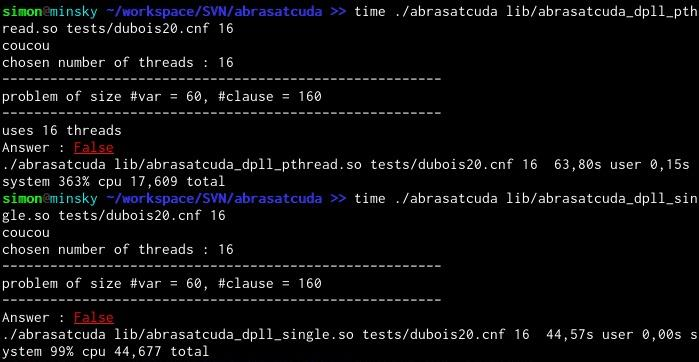
\includegraphics[width = 1.0\textwidth]{./benchmark.jpg}
  \caption[mono-threadé]{Performances comparées des versions à un ou plusieurs threads sur une instance non satisfiable}
  \label{benchmark}
\end{figure}

\begin{figure}[hp]
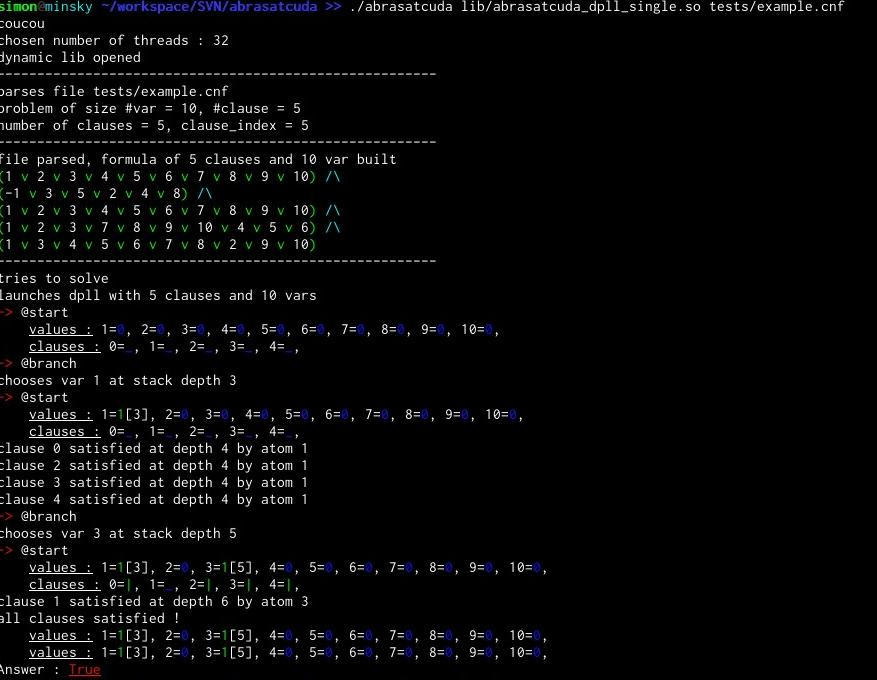
\includegraphics[width = 1.0\textwidth]{./all.jpg}
  \caption[mono-threadé]{Test mono-threadé sur une instance satisfiable}
\end{figure}

On remarque, sur la figure~\ref{multiThread}, que le programme choisit de ne lancer que 4 threads au lieu de 7 comme demandé. Chaque thread a un travail négligeable à fournir puisqu'aucune exploration n'est nécessaire. 

\begin{figure}[hp]
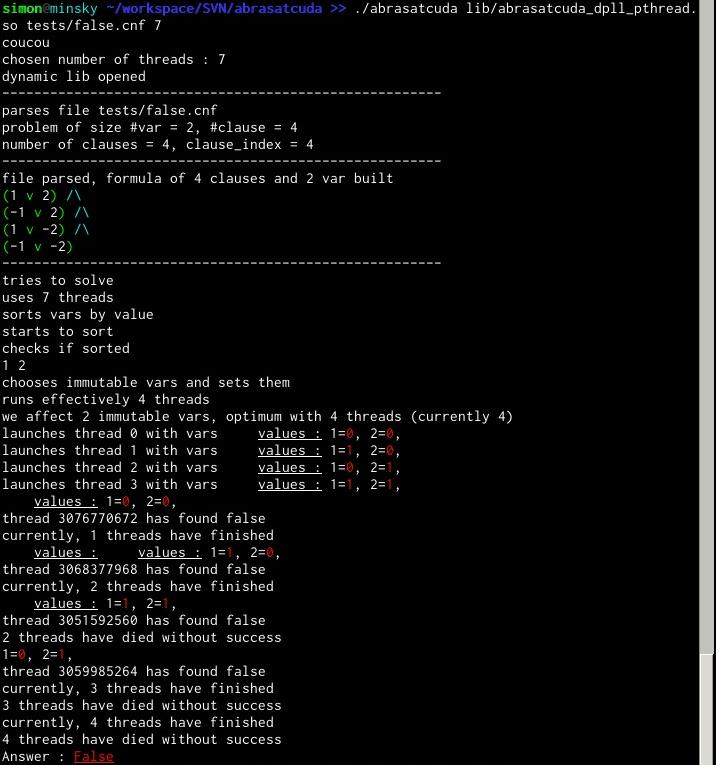
\includegraphics[width = 1.0\textwidth]{./pthread.jpg}
  \caption[multi-threadé]{Test multi-threadé sur une instance non satisfiable}
  \label{multiThread}
\end{figure}
%}}}

\end{document}


